\documentclass{mp}
\renewcommand{\d}[1]{\ensuremath\,\text{d}#1}
\graphicspath{{09_ciagle}}
\subtitle{Zmienne losowe typu ciągłego}
\begin{document}
\frame{\titlepage}
\begin{frame}{Zmienna losowa typu ciągłego}
\[ \forall x\in\R\colon F_X(x)=P(X<x)=\int_{-\infty}^x f(u)\d{u} \]
\begin{block}<2->{Właśności}
\begin{itemize}
\item \[\forall u\in\R\colon f(u)\geq 0\]
\item \[\int_{-\infty}^\infty f(u)\d{u}=1\]
\end{itemize}
\end{block}
\only<3->
{
	\begin{itemize}
	\item<3-> $P(X=x)=\alert<3>{?}$
	\item<4-> $P(a\leq X\leq b)=\alert<4>{?}$
	\end{itemize}
}
\end{frame}
\begin{frame}{Momenty}
\begin{description}
\item[wartość średnia] \[ EX=\int_{-\infty}^\infty xf(x)\d{x} \]
\item<2->[odchylenie standardowe] \[ DX=\sqrt{E(X-EX)^2}\only<3->{=\sqrt{\int_{-\infty}^\infty (x-\mu)^2f(x)\d{x}}} \]
\end{description}
\end{frame}
\begin{frame}{Rozkład jednostajny o parametrach $a<b$}
\only<1>{
	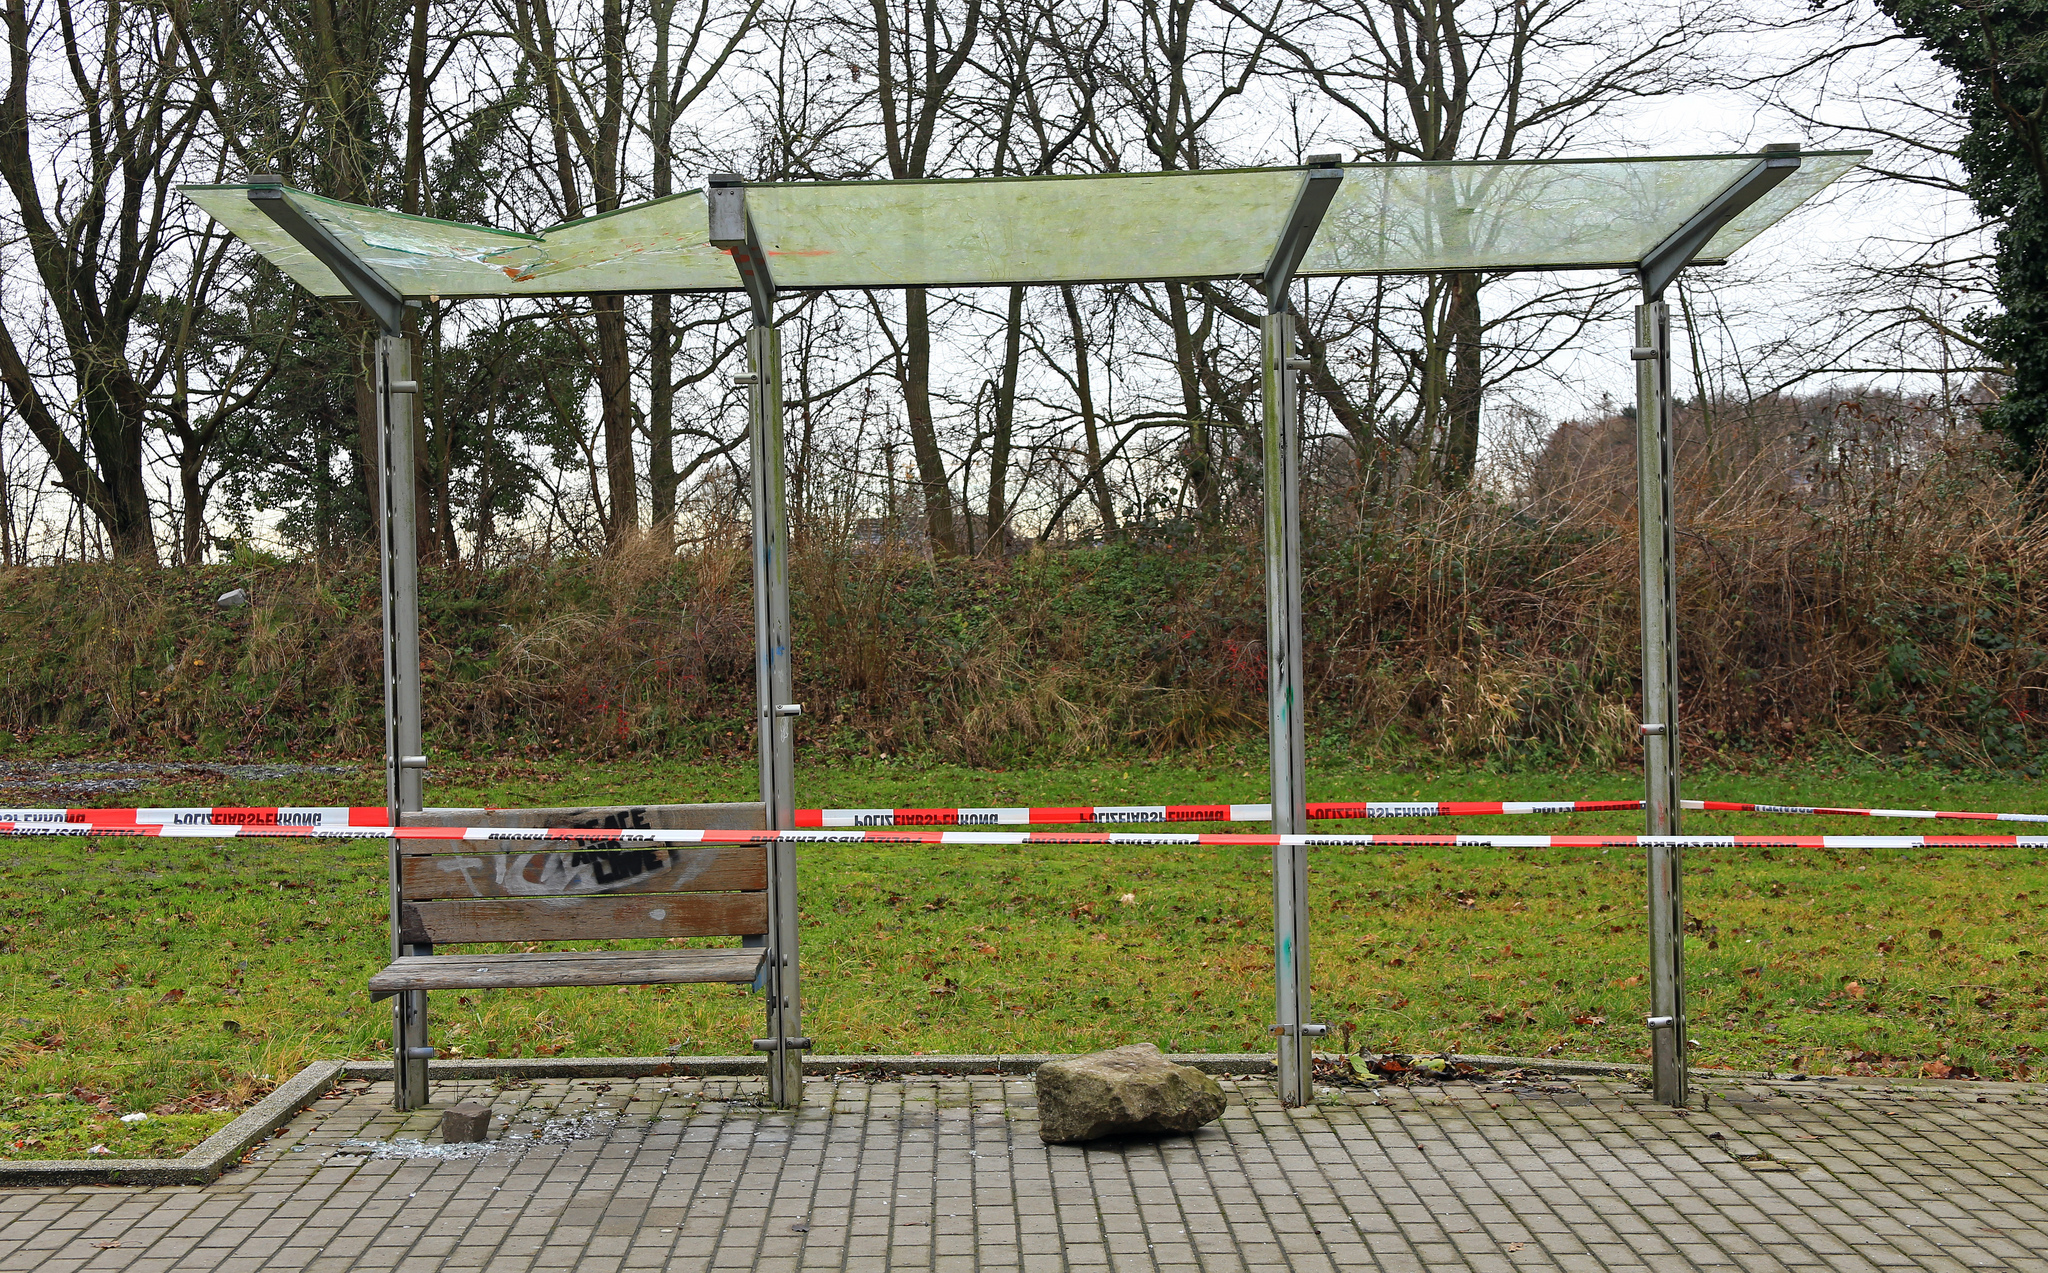
\includegraphics[width=\textwidth]{09_ciagle/bus_stop.jpg}

	{\tiny \url{https://www.flickr.com/photos/hdz/11728759956/} CC-BY-SA 2.0}
}
\only<2->
{
	\begin{columns}[T]
\begin{column}{.6\textwidth}
\begin{tikzpicture}[x=1cm,y=2cm]
\draw[->] (-3,0) -- (4,0) node[right] {$x$};
\draw[->] (0,-.5) -- (0,2) node[above] {$y$};
\draw (-1,0) node[below] {$a$};
\draw (-1,-.05) -- (-1,.05);
\draw (2,0) node[below] {$b$};
\draw (2,-.05) -- (2,.05);
\draw (0,1) node[left] {$1$};
\draw (-.1,1) -- (.1,1);
\draw[color2,thick] (-3,0) -- (-1,0) (-1,.33)--(2,.33) (2,0)--(4,0);
\draw[color4,thick,visible on=<3>] (-3,0) -- (-1,0) (-1,0)--(2,1) (2,1)--(4,1);
\draw[color3,thick,visible on=<4->] (0.5,1.5)--(0.5,-.5);
\fill[color3,semitransparent,visible on=<5->] (-0.366,1.5) rectangle (1.366,-.5);
\end{tikzpicture}
\end{column}
\begin{column}{.39\textwidth}
\begin{gather*}
\textcolor{color2}{f(x)}=\begin{cases} \frac{1}{b-a} \qquad x\in\left<a,b\right> \\ 0 \qquad \text{wpp}\end{cases} \\
\only<3->{\textcolor{color4}{F(x)}=\alert<3>{?}} \\
\only<4->{\textcolor{color3}{EX}=\alert<4>{?}}\\
\only<5->{\textcolor{color3}{DX}=\alert<5>{?}}
\end{gather*}
\end{column}
\end{columns}
}
\end{frame}
\begin{frame}{Rozkład wykładniczy o parametrze $\lambda$}
\only<1>
{
	\def\lambdaval{4}
	\note<1>{Maile przychodzą ze średnią częstotliwością $\lambda=4$}	%miałem tu \lambdaval, ale nie działało
	\center
	\begin{tikzpicture}[x=1.2cm]
	\draw [thick,->] (-.5,0) -- (8.5,0);
	\foreach \h [evaluate=\h as \x using \h-8] in {8,9,...,16}
	{
		\draw [thick] (\x,-.05) -- ++(0,.1) node[anchor=north] {$\h^{00}$};
	}
	\foreach \n [remember=\pgfmathresult as \prevt (initially 0)] in {1,...,50}
	{
		\pgfmathparse{-ln(1-rnd)/\lambdaval+\prevt}
		\pgfmathtruncatemacro{\h}{\pgfmathresult+.5}
		\ifnum \h>7
			\breakforeach
		\fi
		\node at (\pgfmathresult,.25) {
\includegraphics[width=.5cm]{09_ciagle/envelope-35393_640.png}};
	}
	\end{tikzpicture}
	\vfill
	{\tiny{Rysunek koperty z domeny publicznej, \url{http://pixbay.com}, użytkownik \emph{Nemo}}}
}
\only<2->
{
\note<2>{Ciągły odpowiednik rozkładu geometrycznego. Czas pomiędzy zdarzeniami zachodzącymi niezależnie, ze stałą prędkością $\lambda$.}
\begin{columns}[T]
\begin{column}{.5\textwidth}
\begin{tikzpicture}[x=1cm,y=2cm]
\draw[->] (-1,0) -- (4,0) node[right] {$x$};
\draw[->] (0,-.5) -- (0,2) node[above] {$y$};
\draw (0,1) node[left] {$1$} (-.1,1) -- (.1,1);
\draw (0,.5) node[left] {$0{,}5$} (-.1,.5) -- (.1,.5);
\draw (1,0) node[below] {$1$} (1,-.05) -- ++(0,.1);

\draw[color2,thick] (-1,0) -- (0,0);
\draw[color2,thick,domain=0:4,samples=1000] plot (\x,{1.5*exp(-1.5*\x)});
\draw[color4,thick,domain=0:4,samples=1000,visible on=<2->] plot (\x,{1-exp(-1.5*\x)});
\draw[color4,thick,visible on=<2->] (-1,0) -- (0,0);
\draw[color3,thick,visible on=<3->] (.67,-.25) -- (.67,1.75);
\fill[color3,semitransparent,visible on=<4->] (0,-.25) rectangle (1.33,1.75);
\end{tikzpicture}
\end{column}
\begin{column}{.49\textwidth}
\begin{gather*}
\textcolor{color2}{f(x)}=\begin{cases} \lambda e^{-\lambda x} & x\in\left<0,\infty\right) \\ 0 & \text{wpp} \end{cases}\\
\only<2->{\textcolor{color4}{F(x)}=\alert<2>{?}} \\
\only<3->{\textcolor{color3}{EX}=\frac{1}{\lambda}}\\
\only<4->{\textcolor{color3}{DX}=\frac{1}{\lambda}} \\
\only<5->{P(X>a+b|X>a)=P(X>b)}
\end{gather*}
\end{column}
\end{columns}
}
\end{frame}
\begin{frame}{Rozkład normalny (Gaussa) $N(\mu,\sigma)$}
\begin{minipage}{.54\textwidth}
\begin{tikzpicture}[x=1cm,y=5cm]
%TODO: fajnie by było to sparametryzować i móc robić różne rozkłady normalne w ten sposób
\draw[->] (-4,0) -- (4,0) node[right] {$x$};
\draw[->] (0,-.2) -- (0,1.2) node[above] {$y$};
\draw (0,1) node[left] {$1$} (-.1,1) -- (.1,1);
\draw (0,.5) node[left] {$0{,}5$} (-.1,.5) -- (.1,.5);
\draw (1,0) node[below] {$1$};
\draw (1,-.02) -- (1,.02);
\draw[color2,thick,domain=-4:4,samples=1000] plot (\x,{exp((-((\x)^2))/2)/sqrt(2*pi)});
\draw[color4,visible on=<2->,thick] (-4,0)
\foreach \n in {-400,...,400}
{
	\pgfextra{\pgfmathparse{exp((-((\n/100)^2))/2)/sqrt(2*pi)/100}}
	-- ++(.01,\pgfmathresult)
};

\draw[color3,very thick,visible on=<3->] (0,1)--(0,-.1);
\fill[color3,semitransparent,visible on=<4->] (-1,1) rectangle (1,-.1);
\end{tikzpicture}
\end{minipage}
\begin{minipage}{.45\textwidth}
\begin{gather*}
\textcolor{color2}{f(x)}=\frac{1}{\sigma\sqrt{2\pi}}\exp\left(\frac{-(x-\mu)^2}{2\sigma^2}\right) \\
\only<2->{\textcolor{color4}{F(x)}=\int_{-\infty}^x f(x)\d{x}} \\
\only<3->{\textcolor{color3}{EX}=\mu} \\
\only<4->{\textcolor{color3}{DX}=\sigma}
\end{gather*}
\end{minipage}
\end{frame}
\begin{frame}{Standardowy rozkład normalny $N(0,1)$}
\small
\tabcolsep=0.1cm
\input{gauss.tex}
\note{Odczytać/obliczyć:
\[P(X\leq 0{,}83) \qquad P(X\geq 1{,}24) \qquad P(X\leq -0{,}83\]
}
\end{frame}
\begin{frame}{Dwuwymiarowe zmienne losowe typu ciągłego}
\begin{gather*}
\forall x,y\in\R\colon F_{X,Y}(x,y)=P(X<x,Y<y)=\int_{-\infty}^x\int_{-\infty}^y f(u,v)\d{v}\d{u} \\
\only<2->
{
	f_X(x)=\int_{-\infty}^\infty f(x,v)\d{v} \qquad F_X(x)=F_{X,Y}(x,\infty) \\
}
\only<3->
{
	f_Y(y)=\int_{-\infty}^\infty f(u,y)\d{u} \qquad F_Y(y)=F_{X,Y}(\infty,y) \\
}
\end{gather*}
%TODO: to raczej gdzies w 05_zmienne.tex
%\only<4>
%{
%	\alert{Jak obliczyć $P(a\leq X< b,c\leq Y<d)$ mając do dyspozycji wyłącznie dystrybuantę?}
%}
\end{frame}
\end{document}
